\documentclass[tikz,border=7pt]{standalone}
\usepackage{amsmath}
\usetikzlibrary{arrows.meta,positioning}

\tikzset{
  comp/.style={
    draw,rectangle,rounded corners=2pt,
    minimum width=36mm,minimum height=26mm,align=center
  },
  signal/.style={-{Latex[length=2.1mm]},thick}
}

\begin{document}
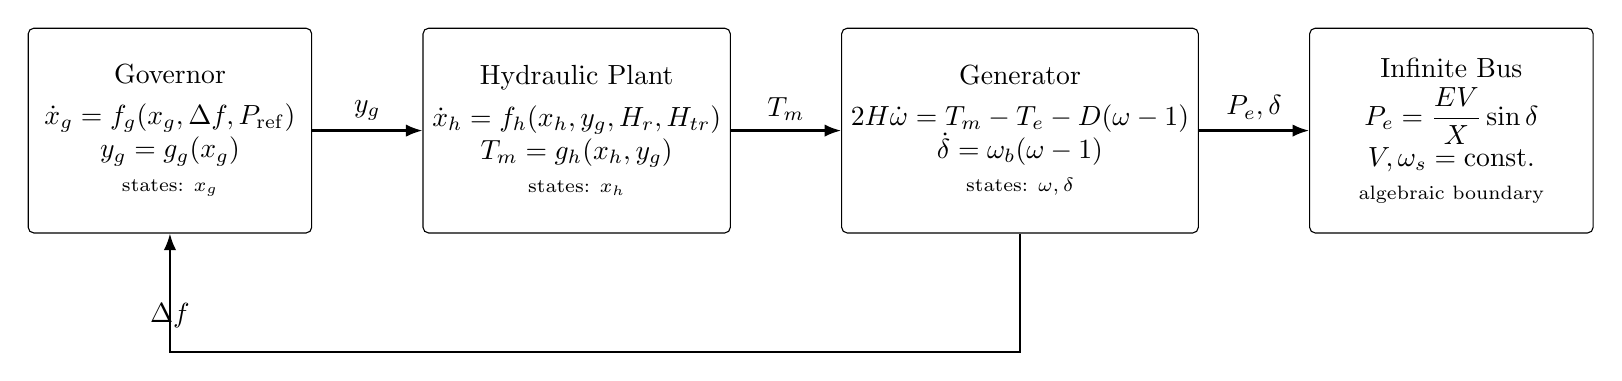
\begin{tikzpicture}[node distance=14mm]

\node[comp] (gov) {
Governor\\[1mm]
$\dot x_g=f_g(x_g,\Delta f,P_{\rm ref})$\\
$y_g=g_g(x_g)$\\
\scriptsize states: $x_g$
};

\node[comp,right=of gov] (hyd) {
Hydraulic Plant\\[1mm]
$\dot x_h=f_h(x_h,y_g,H_r,H_{tr})$\\
$T_m=g_h(x_h,y_g)$\\
\scriptsize states: $x_h$
};

\node[comp,right=of hyd] (gen) {
Generator\\[1mm]
$2H\dot\omega=T_m-T_e-D(\omega-1)$\\
$\dot\delta=\omega_b(\omega-1)$\\
\scriptsize states: $\omega,\delta$
};

\node[comp,right=of gen] (grid) {
Infinite Bus\\[1mm]
$P_e=\dfrac{EV}{X}\sin\delta$\\
$V,\omega_s=\mathrm{const.}$\\
\scriptsize algebraic boundary
};

\draw[signal] (gov) -- node[above] {$y_g$} (hyd);
\draw[signal] (hyd) -- node[above] {$T_m$} (gen);
\draw[signal] (gen) -- node[above] {$P_e,\delta$} (grid);

\draw[signal] (gen.south) |- ++(0,-15mm)
  -| node[pos=0.75,below] {$\Delta f$} (gov.south);

\end{tikzpicture}
\end{document}
